\documentclass[portrait,a1paper,fontscale=0.42]{baposter}
% \documentclass[landscape,a0paper,fontscale=0.292]{baposter}

\usepackage[T1]{fontenc} %% set font encode
\usepackage[utf8]{inputenc}
\usepackage[unicode]{hyperref}
\usepackage{vntex}
\usepackage[vietnamese=nohyphenation]{hyphsubst} % fix warning when using vietnamese babel
\usepackage[english, vietnamese]{babel}
\usepackage{amssymb}
\usepackage[vlined]{algorithm2e}
\usepackage{times}
\usepackage{calc}
\usepackage{url}
\usepackage{graphicx}
% \usepackage{tikz}
\usepackage{pgf}
\usepackage{pgfpages}
\usepackage{amsmath}
\usepackage{amssymb}
\usepackage{commath}
\usepackage{relsize}
\usepackage{multirow}
\usepackage{booktabs}
\usepackage{mathtools}
\usepackage{graphicx}

\usepackage{multicol}
% \setlength{\columnsep}{10em} % Slightly increase the space between columns
% \setlength{\columnseprule}{0mm} % No horizontal rule between columns
\usepackage{makecell}

\usepackage{tabulary}
\usepackage{ae}
\usepackage{enumitem}
\usepackage{caption}
\usepackage{colortbl}
\usepackage{xcolor}

\graphicspath{{images/}}
\usepackage{float}
\setlist[itemize]{leftmargin=*,nosep}
\setlength{\columnsep}{0.7em}
\setlength{\columnseprule}{0mm}

\pgfpagesdeclarelayout{boxed}
{
    \edef\pgfpageoptionborder{0pt}
}
{
    \pgfpagesphysicalpageoptions
    {
        logical pages=1,
    }
    \pgfpageslogicalpageoptions{1}
    {
        border code=\pgfsetlinewidth{10pt}\pgfstroke,%
        border shrink=\pgfpageoptionborder,%
        resized width=.99\pgfphysicalwidth,%
        resized height=.99\pgfphysicalheight,%
        center=\pgfpoint{.5\pgfphysicalwidth}{.5\pgfphysicalheight}%
    }%
}
% Draw page border
\pgfpagesuselayout{boxed}

\DeclareMathOperator{\Expected}{\mathbb{E}}

% %%%%%%%%%%%%%%%%%%%%%%%%%%%%%%%%%%%%%%%%%%%%%%%%%%%%%%%%%%%%%%%%%%%%%%%%%%%%%%%%
% % Save space in lists. Use this after the opening of the list
% %%%%%%%%%%%%%%%%%%%%%%%%%%%%%%%%%%%%%%%%%%%%%%%%%%%%%%%%%%%%%%%%%%%%%%%%%%%%%%%%
\newcommand{\compresslist}{%
    \setlength{\itemsep}{0pt}%
    \setlength{\parskip}{0pt}%
    \setlength{\parsep}{0pt}%
}
\renewcommand{\rmdefault}{ptm} % Arial
\renewcommand{\sfdefault}{ptm} % Arial

%%%%%%%%%%%%%%%%%%%%%%%%%%%%%%%%%%%%%%%%%%%%%%%%%%%%%%%%%%%%%%%%%%%%%%%%%%%%%
%% Begin of Document
%%%%%%%%%%%%%%%%%%%%%%%%%%%%%%%%%%%%%%%%%%%%%%%%%%%%%%%%%%%%%%%%%%%%%%%%%%%%%
\begin{document}
%% Here starts the poster
%%---------------------------------------------------------------------------
\begin{poster}
    {
        % % Show grid to help with alignment
        % grid=true,
        columns=2,
        % rows=10, 
        % % Column spacing
        % colspacing=0.8em,
        % % rowspacing=0.3em,
        % % Format background
        % background=plain,%none,
        % bgColorOne=white,
        % bgColorTwo=yellow!50!white,%cyan!10!white,
        % % Color style
        % borderColor=cyan!30!white!90!black,
        % % Format of textbox
        % textborder=roundedsmall,%faded,
        % % Format header
        % % headerColorOne=white,%cyan!20!white!90!black,
        % % headerColorTwo=blue,
        % headerheight=0.12\textheight,
        % %% Format of text header
        % headerborder=closed,%open,
        % headershape=smallrounded,%roundedright,
        % headershade=shade-tb-inverse,%plain,
        headerborder=closed, % Adds a border around the header of content boxes
        colspacing=1em, % Column spacing
        bgColorOne=white, % Background color for the gradient on the left side of the poster
        bgColorTwo=white, % Background color for the gradient on the right side of the poster
        borderColor=cyan!70!white, % Border color
        headerColorOne=cyan!30!white, % Background color for the header in the content boxes (left side)
        headerColorTwo=white, % Background color for the header in the content boxes (right side)
        headerFontColor=white, % Text color for the header text in the content boxes
        boxColorOne=yellow!03!white, % Background color of the content boxes
        textborder=roundedsmall, % Format of the border around content boxes, can be: none, bars, coils, triangles, rectangle, rounded, roundedsmall, roundedright or faded
        eyecatcher=true, % Set to false for ignoring the left logo in the title and move the title left
        headerheight=0.1\textheight, % Height of the header
        headershape=smallrounded, % Specify the rounded corner in the content box headers, can be: rectangle, small-rounded, roundedright, roundedleft or rounded
        headerfont=\Large\bf\textsc, % Large, bold and sans serif font in the headers of content boxes
        %textfont={\setlength{\parindent}{1.5em}}, % Uncomment for paragraph indentation
        linewidth=1.5pt % Width of the border lines around content boxes
    }
    % Eye Catcher
    {
        % 
\includegraphics[width=0.08\linewidth]{Medical_CT_poster/images/LogoBK.jpg}
        % \makebox[0.03\textwidth]{} 
        % 
\includegraphics[width=0.08\linewidth]{Medical_CT_poster/images/qr_137291.png}
    }
    % Title
    {
        \vspace{0.05em} 
        \color{blue} \sc\huge\bf Hệ thống làm nhãn cho ảnh chụp cắt lớp vi tính (CT)\\ với sự trợ giúp của Trí tuệ nhân tạo
    }
    % Authors
    {
        \vspace{0.4em} 
        Cao Thanh Tùng (1613989) - Nguyễn Thanh Tuấn (1613907) - Phan Ngọc Thịnh (1613361)\\[0.2em]
        GVHD: TS. Lê Thành Sách - TS. Nguyễn Hồ Mẫn Rạng\\[0.2em]
        {Đại học Bách Khoa Thành phố Hồ Chí Minh - Khoa Khoa học và Kỹ thuật Máy tính\\[2.5em]}
    }
    % University Logo
    {
        
\includegraphics[width=0.15\linewidth]{Medical_CT_poster/images/LogoBK.jpg}\\[2.5em]
    }
%%%%%%%%%%%%%%%%%%%%%%%%%%%%%%%%%%%%%%%%%%%%%%%%%%%%%%%%%%%%%%%%%%%%%%%%%%%%%%
%%% Now define the boxes that make up the poster
%%%---------------------------------------------------------------------------
%%% Each box has a name and can be placed absolutely or relatively.
%%% The only inconvenience is that you can only specify a relative position 
%%% towards an already declared box. So if you have a box attached to the 
%%% bottom, one to the top and a third one which should be in between, you 
%%% have to specify the top and bottom boxes before you specify the middle 
%%% box.
%%%%%%%%%%%%%%%%%%%%%%%%%%%%%%%%%%%%%%%%%%%%%%%%%%%%%%%%%%%%%%%%%%%%%%%%%%%%%%
\headerbox{\bf\color{blue} Giới thiệu đề tài}{name=abstract,column=0,row=0,span=1}{
    \textbf{\color{blue} Động lực thực hiện}
    \begin{itemize}
    \setlength{\itemsep}{10pt}
    \setlength{\parskip}{10pt}
    \compresslist
    \setlength{\itemindent}{.2in}
        \item Tỉ lệ tử vong do ung thư gan tại Việt Nam cao.
        \item Ứng dụng trí tuệ nhân tạo vào lĩnh vực y học trở nên phổ biến.
    \end{itemize}
    
    \textbf{\color{blue} Ý nghĩa thực tiễn}
    \begin{itemize}
    \compresslist
     \setlength{\itemindent}{.2in}
        \item Giúp bác sĩ chẩn đoán bệnh nhanh chóng và chính xác hơn.
        \item Giải quyết vấn đề thiếu dữ liệu ảnh y khoa nhờ hệ thống làm nhãn.
    \end{itemize}
    
    \textbf{\color{blue} Mục tiêu và phạm vi}
    \begin{itemize}
    \compresslist
    \setlength{\itemindent}{.2in}
        \item Phân đoạn gan.
        \item Phân đoạn mạch máu.
        \item Kế thừa và phát triển hệ thống làm nhãn ảnh y khoa DAT.
    \end{itemize}
}

%%%%%%%%%%%%%%%%%%%%%%%%%%%%%%%%%%%%%%%%%%%%%%%%%%%%%%%%%%%%%%%%%%%%%%%%%%%%%
\headerbox{\bf\color{blue} Thách thức}{name=challenge,column=0, row=1, below=abstract,     span=1}{
	\begin{minipage}[t]{0.5\linewidth}
	    \vspace{-6mm}
        \begin{figure}[H]
        \centering
        	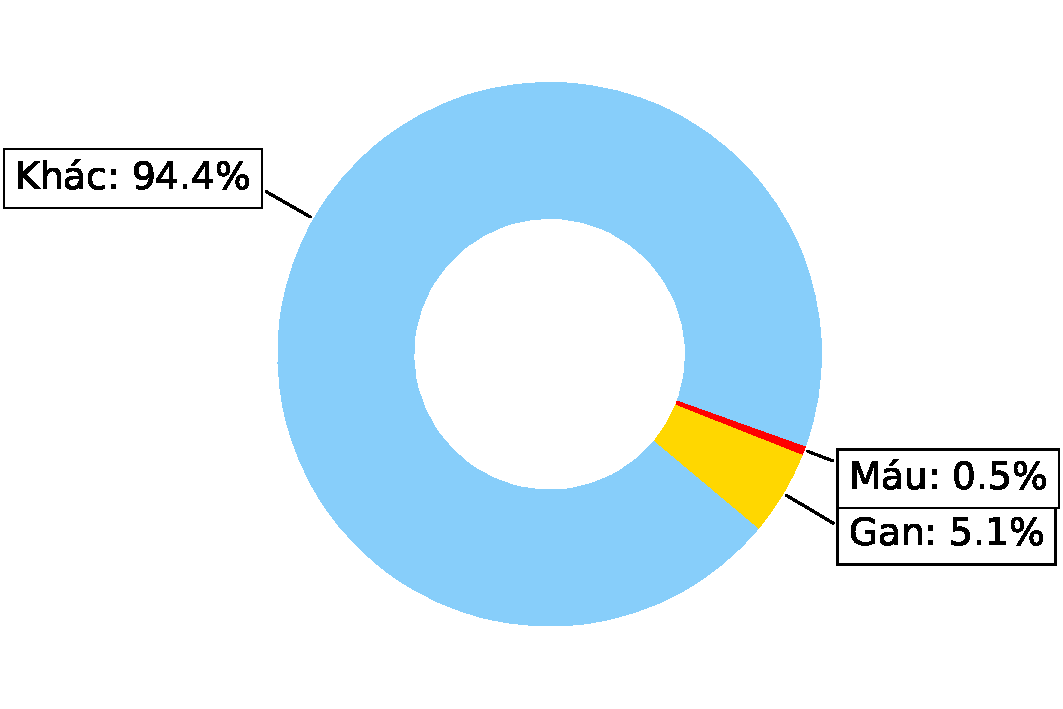
\includegraphics[width=\linewidth]{Medical_CT_poster/images/challenge/liver-vessel-bg-ratio.pdf}
        	\vspace{-8mm}
        	\caption*{Tỉ lệ gan, mạch máu trong ảnh CT.}
        \end{figure}
        \vspace{-0.45cm}
        \begin{itemize}
            \compresslist
            \item Hạn chế về số lượng dữ liệu.
    		\item Mất cân bằng dữ liệu.
        \end{itemize}   
	\end{minipage}
	\hfill
	\begin{minipage}[t]{0.4\linewidth}
	    \vspace{-5mm}
	    \begin{figure}[H]
        \centering
            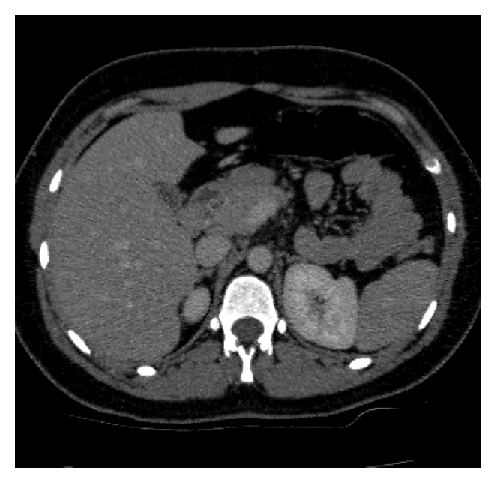
\includegraphics[width=.8\linewidth]{Medical_CT_poster/images/challenge/ct-low-constrast.pdf}
            \vspace{-2mm}
            \caption*{Một lát cắt ảnh CT gan.}
	    \end{figure}
	    \vspace{-0.45cm}
	    \begin{itemize}
        \compresslist
            \item Độ tương phản thấp.
			\item Chi phí tính toán cao.
        \end{itemize}   
	\end{minipage}
}

%%%%%%%%%%%%%%%%%%%%%%%%%%%%%%%%%%%%%%%%%%%%%%%%%%%%%%%%%%%%%%%%%%%%%%%%%%%%%
\headerbox{\bf\color{blue} Mô hình đề xuất}{name=proposed_model,column=1,row=0,span=1}{
    \vspace{-5mm}
    \begin{align}
        \nonumber
        Loss = \mu_{1}Loss_{s1} + \mu_{2}Loss_{s2} + \mu_{3}Loss_{main}
    \end{align}
    \vspace{-10mm}
    \begin{figure}[H]
        \centering
		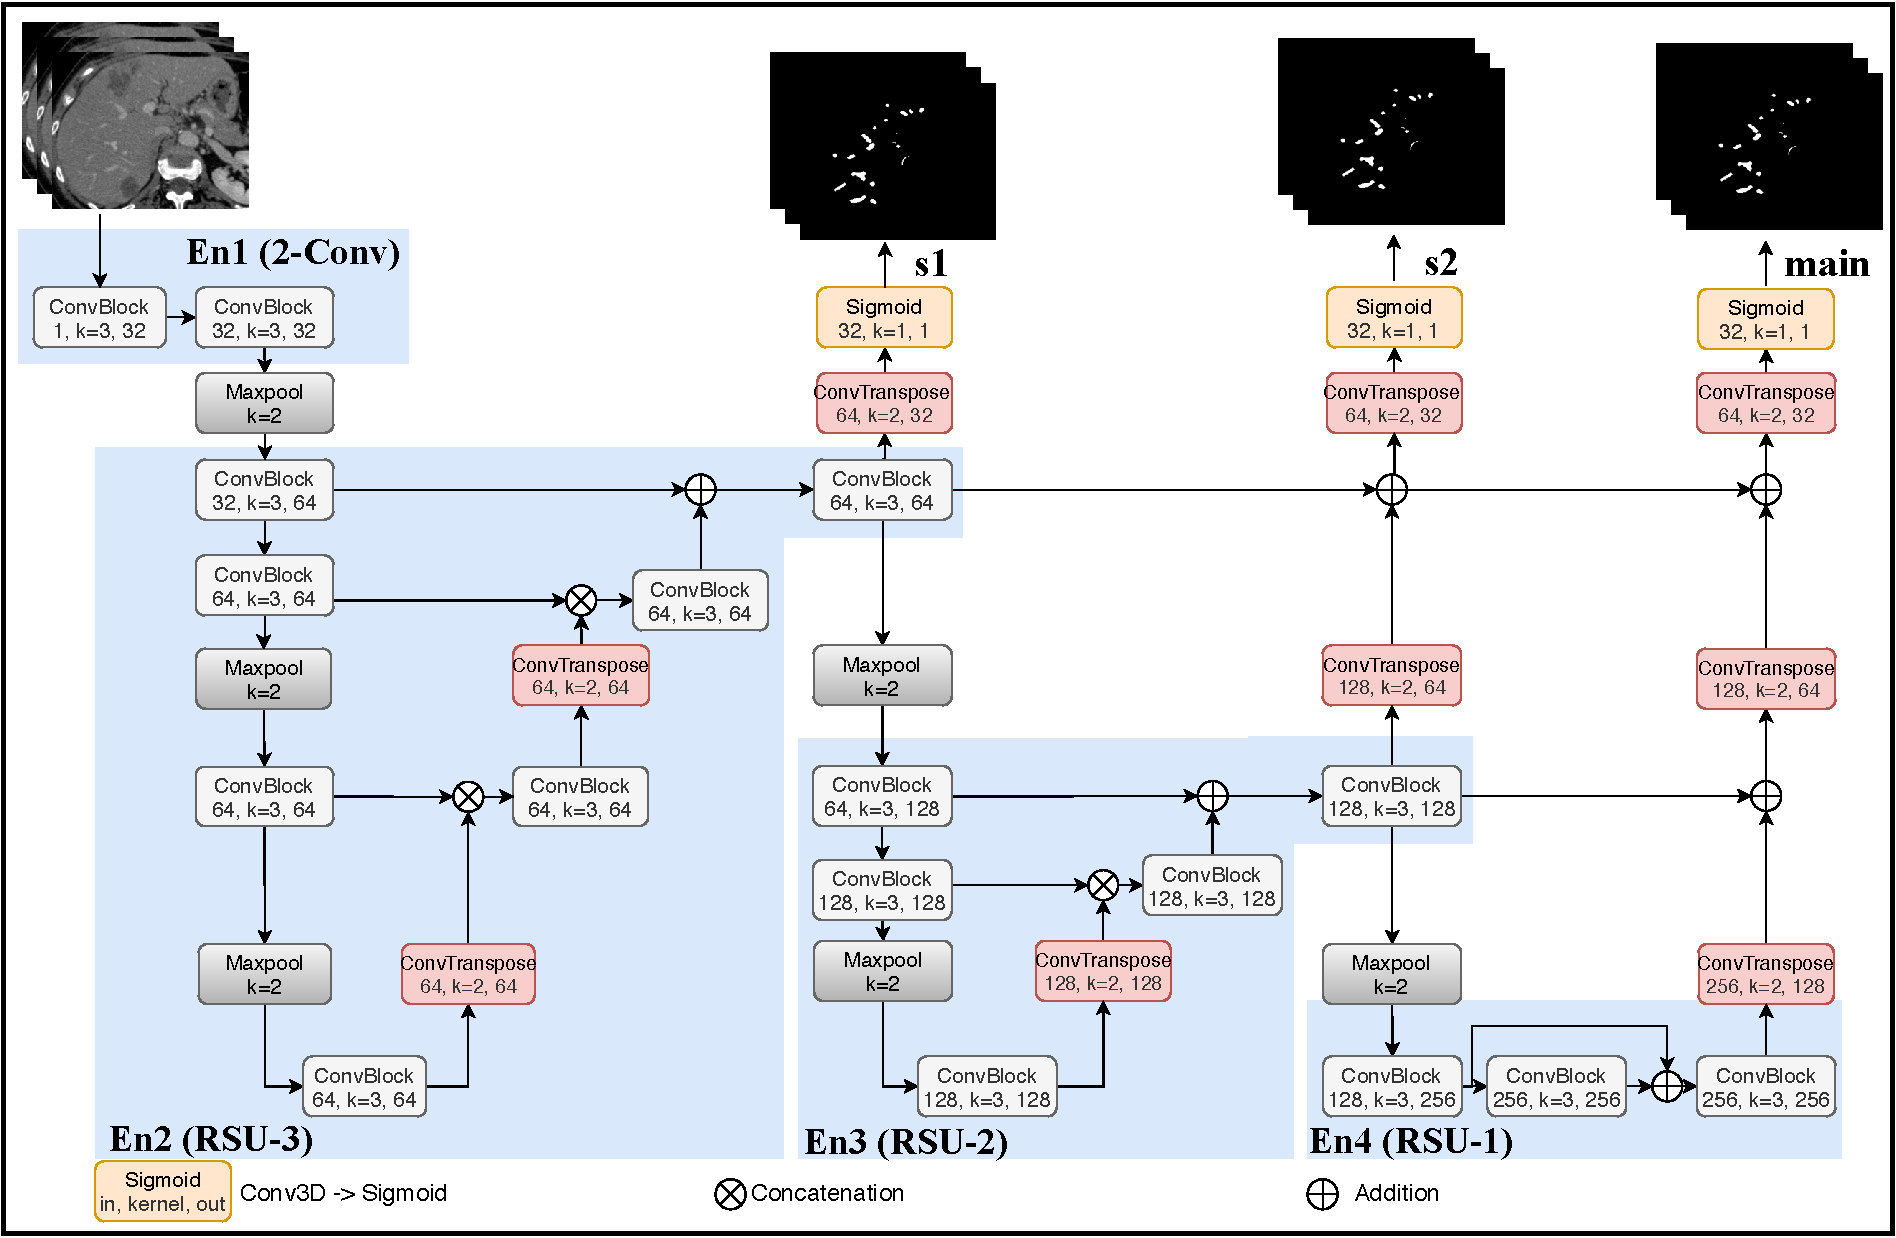
\includegraphics[width=0.99\textwidth]{Medical_CT_poster/images/proposed/u2net3d_arch.pdf}
		\vspace{-3mm}
		\caption*{Kiến trúc mô hình đề xuất U2net3D*}
	\end{figure}
}
%%%%%%%%%%%%%%%%%%%%%%%%%%%%%%%%%%%%%%%%%%%%%%%%%%%%%%%%%%%%%%%%%%%%%%%%%%%%%
\headerbox{\bf\color{blue} Thí nghiệm và kết quả}{name=experiment_result,column=1,row=1,below=proposed_model,span=1}{
    \textbf{\color{blue} Kết quả trên mạch máu}
    \vspace{-3mm}
    \begin{table}[H]
    \renewcommand{\arraystretch}{1.1}
    \centering
    \begin{tabular}{c l c c c}
        \Xhline{2\arrayrulewidth}
        {\textbf{STT}} & {\textbf{Mô hình}} & \textbf{Dice} & \textbf{Recall} & \textbf{Precision} \\ 
        \Xhline{2\arrayrulewidth}
        1   & Unet2D\small[\textcolor{blue}{1}]       & 41.17 & 60.05 & 31.32\\
        2   & Unet3D\small[\textcolor{blue}{2}]       & 56.29 & 44.27 & \textbf{73.97} \\
        3   & CNN3D\small[\textcolor{blue}{3}]        & 54.26 & 54.98 & 59.16 \\
        4   & U2net3D*     & \textbf{60.75} & \textbf{66.87} & 59.73 \\
        \Xhline{2\arrayrulewidth}
    \end{tabular}
    \vspace{-2mm}
    \caption*{Kết quả phân đoạn mạch máu của các mô hình (\%).}
    \end{table}
    \vspace{-6mm}
    \begin{figure}[H]
		\centering
	    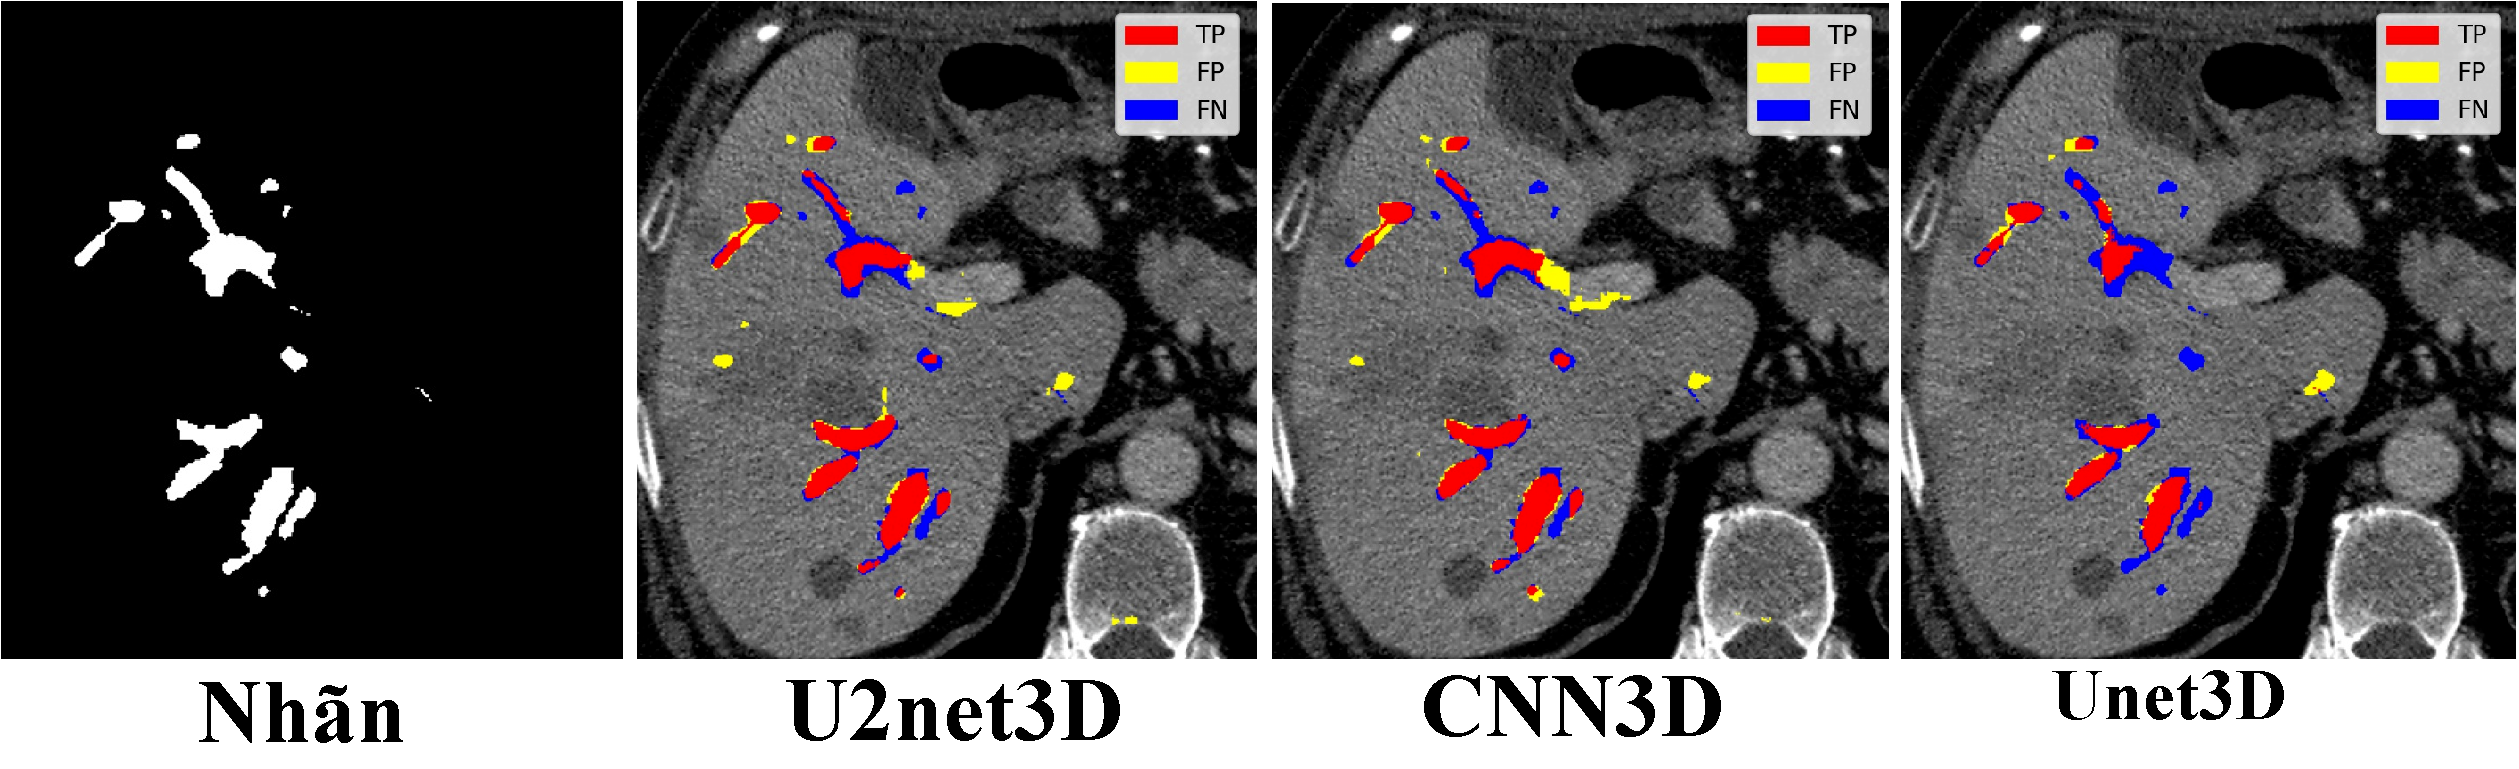
\includegraphics[width=0.85\textwidth]{Medical_CT_poster/images/result/vis_result.pdf}
	    \vspace{-3mm}
		\caption*{Kết quả phân đoạn mạch máu một lát cắt trên tập 3DIRCADb.}
	\end{figure}
    \vspace{-3mm}
    \textbf{\color{blue} Kết quả trên gan}
    \vspace{-2mm}
    \begin{table}[H]
    \centering
    \begin{tabular}{c c c c c c}
    \Xhline{3\arrayrulewidth}
    {\textbf{STT}} & {\textbf{Mô hình}} & \textbf{Dice} & \textbf{Recall} & \textbf{VOE} & \textbf{VD}\\ \hline
    1 & Unet3D\small[\textcolor{blue}{2}]   & 91.82   & 91.54     & 14.53  & 6.37  \\
    2 & CNN3D\small[\textcolor{blue}{3}]    & 95.17   & 94.42     & 9.11   & -1.64  \\
    3 & TLUnet3D\small[\textcolor{blue}{4}]        & 95.70   & \textbf{95.40}     & 8.16   & \textbf{-0.67}    \\
    4 & U2net3D* & \textbf{95.83}  & 95.29 & \textbf{7.9}  & -1.21 \\ 
    \Xhline{3\arrayrulewidth}
    \end{tabular}
    \vspace{-2mm}
    \caption*{Kết quả phân đoạn gan của các mô hình (\%).}
    \end{table}
    \vspace{-6mm}
    \begin{figure}[H]
        \centering
        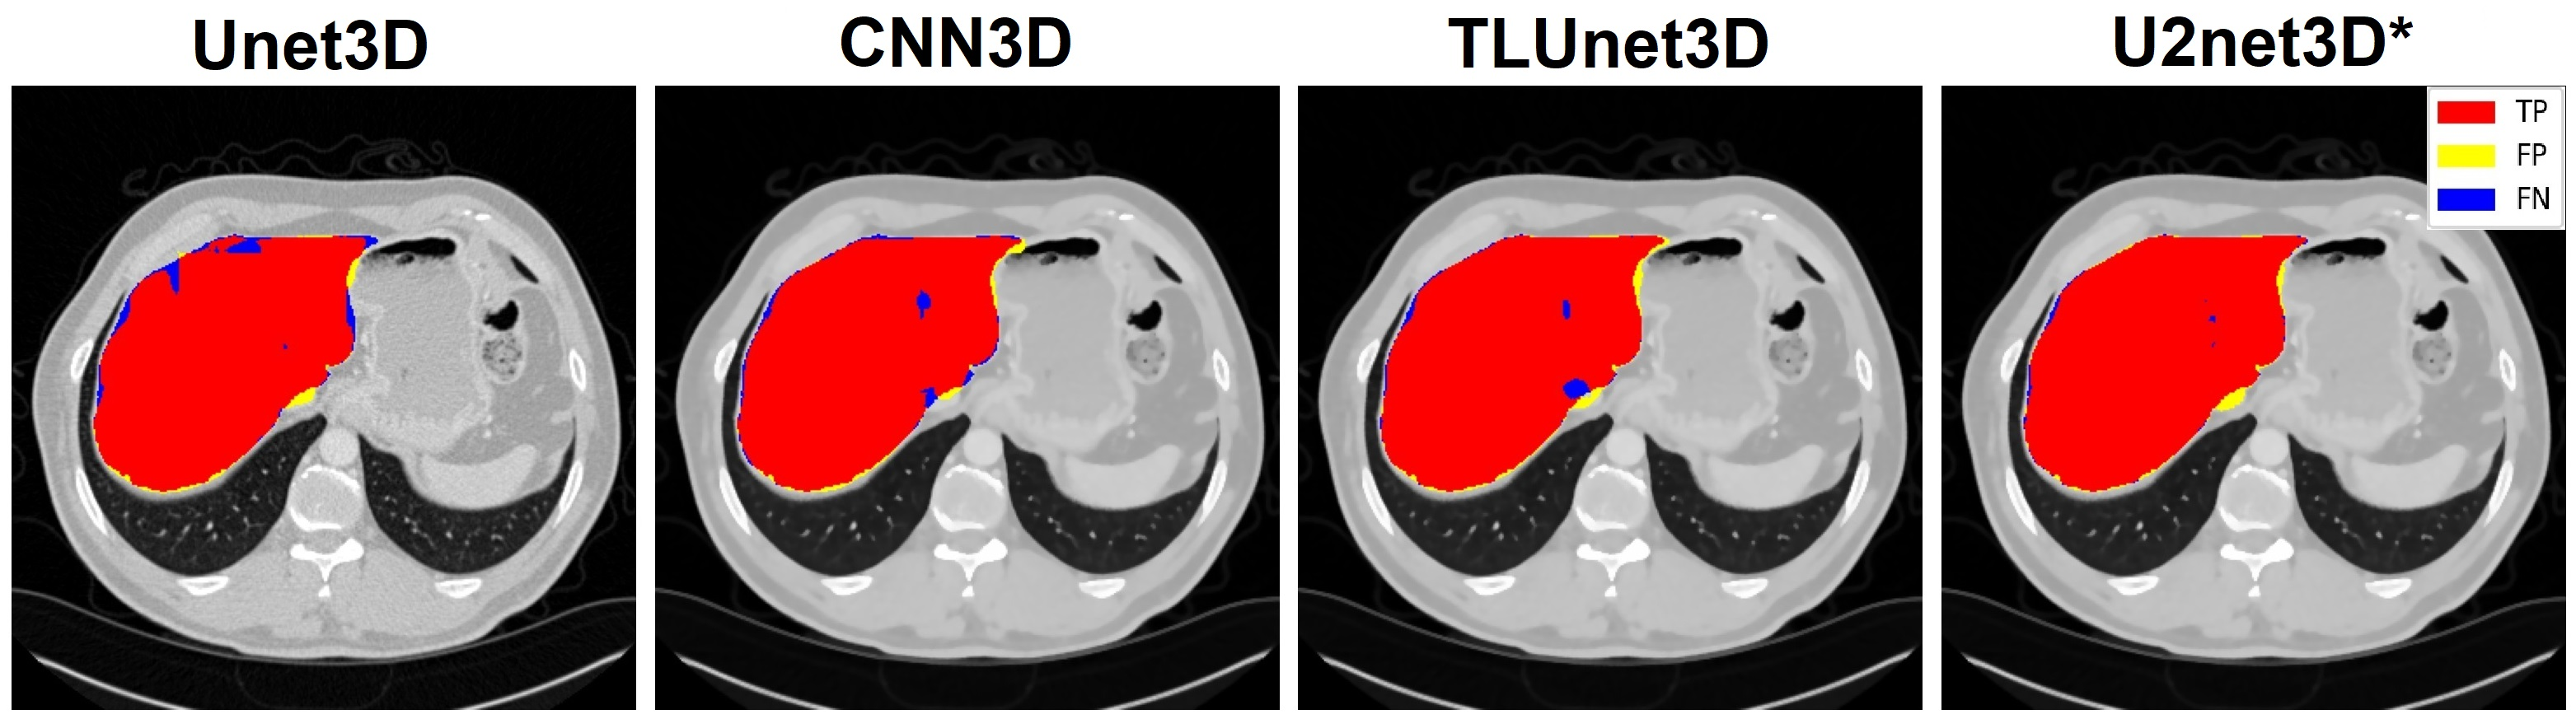
\includegraphics[width=0.85\textwidth]{Medical_CT_poster/images/result/liver-result-legend.jpg}
        \vspace{-3mm}
        \caption*{Kết quả phân đoạn gan một lát cắt trên tập Sliver07.}
    \end{figure}
        
}

%%%%%%%%%%%%%%%%%%%%%%%%%%%%%%%%%%%%%%%%%%%%%%%%%%%%%%%%%%%%%%%%%%%%%%%%%%%%%
\headerbox{\bf\color{blue} Kiến trúc hệ thống Data Annotation Tool}{name=architecture, column=0, row=2, below=challenge,   span=1}{
    \vspace{-5mm}
	\begin{minipage}[t]{0.99\linewidth}
        \begin{figure}[H]
        \centering
        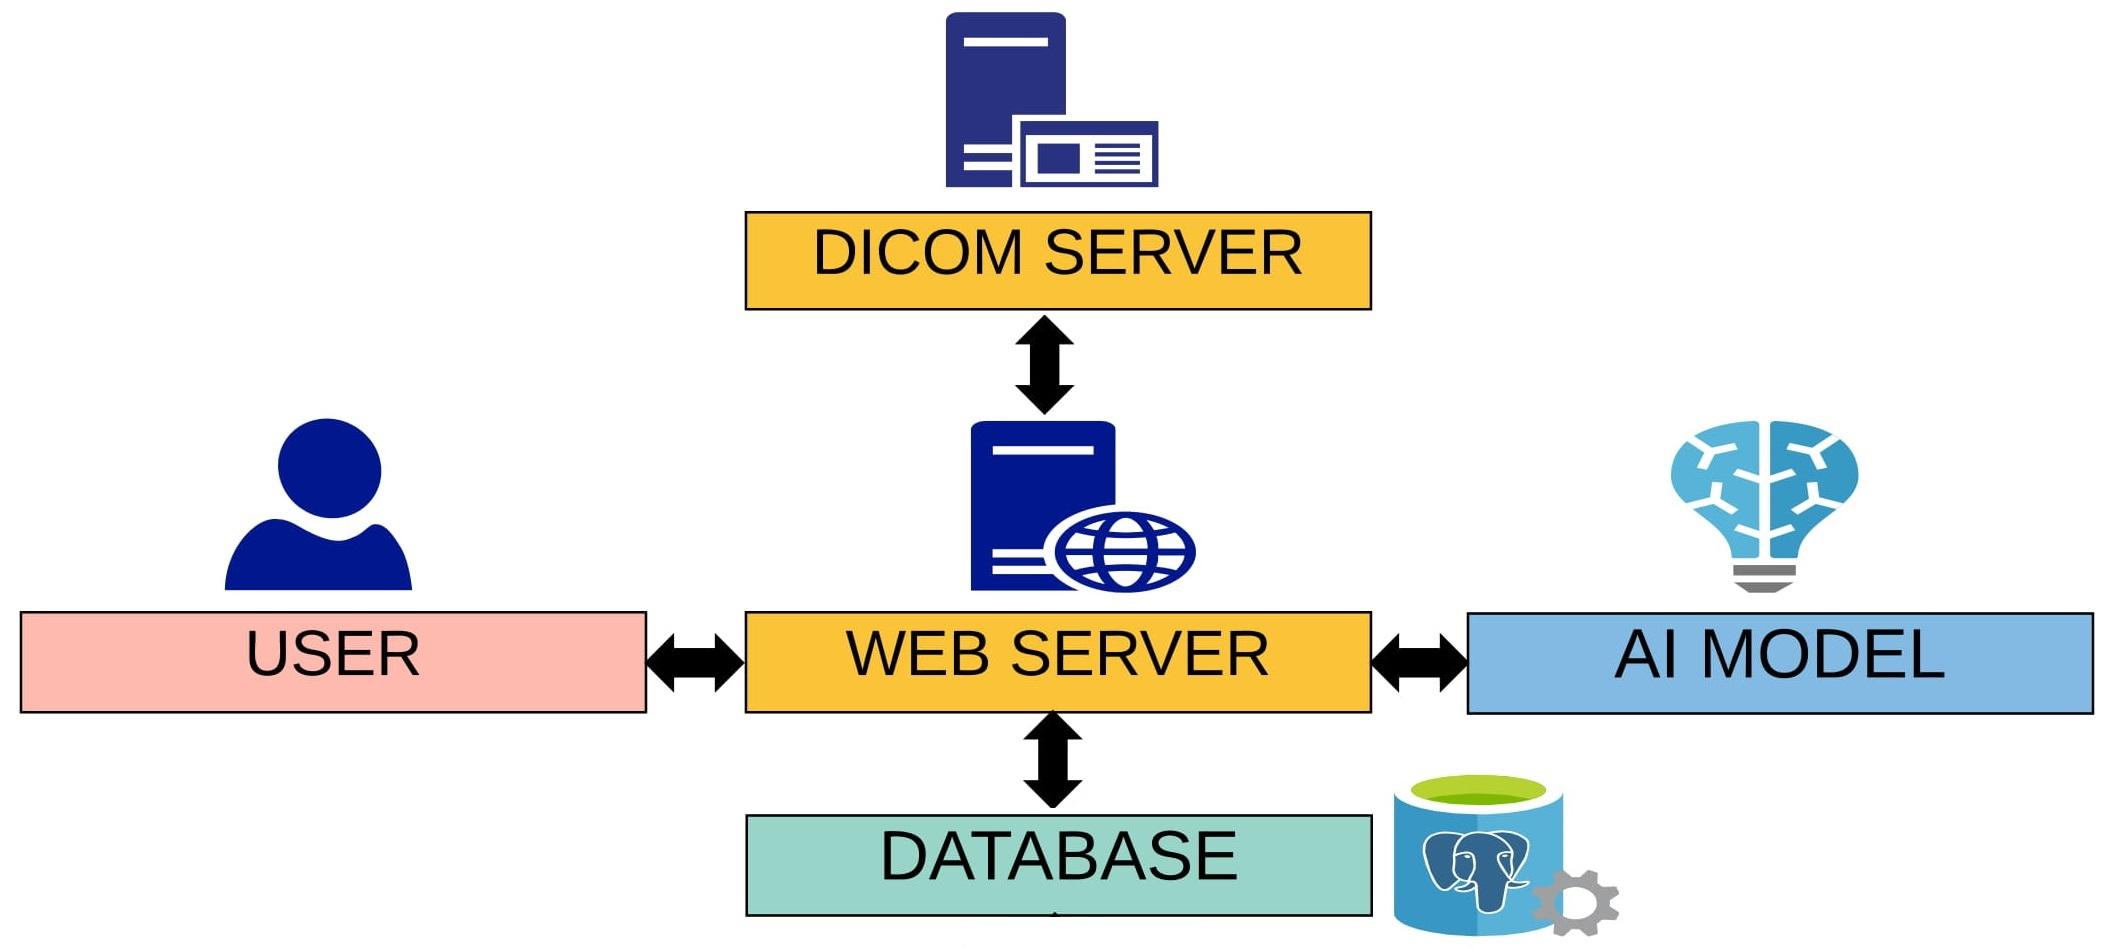
\includegraphics[width=\textwidth]{Medical_CT_poster/images/DAT/mvt-2.jpg}
        \vspace{-7mm}
        \caption*{Tổng quan kiến trúc hệ thống làm nhãn ảnh y khoa DAT.}
        \end{figure}
	\end{minipage}
	\hfill
}

\headerbox{\bf\color{blue} Giao diện ứng dụng DAT}{name=gui, column=0, row=3, below=architecture,  span=1}{
    \vspace{1mm}
    \begin{itemize}[topsep=6pt,itemsep=4pt,partopsep=4pt, parsep=4pt]
        \compresslist
        \setlength{\itemindent}{.3in}
        \item Tích hợp dự đoán AI và giải thuật tăng trưởng vùng theo mức xám.
        \item Vẽ bằng bút, vẽ tự do, kéo thả, hiển thị theo đường biên.
    \end{itemize}
    \vspace{-10mm}
	\begin{minipage}[t]{0.99\linewidth}
        \begin{figure}[H]
        \centering
        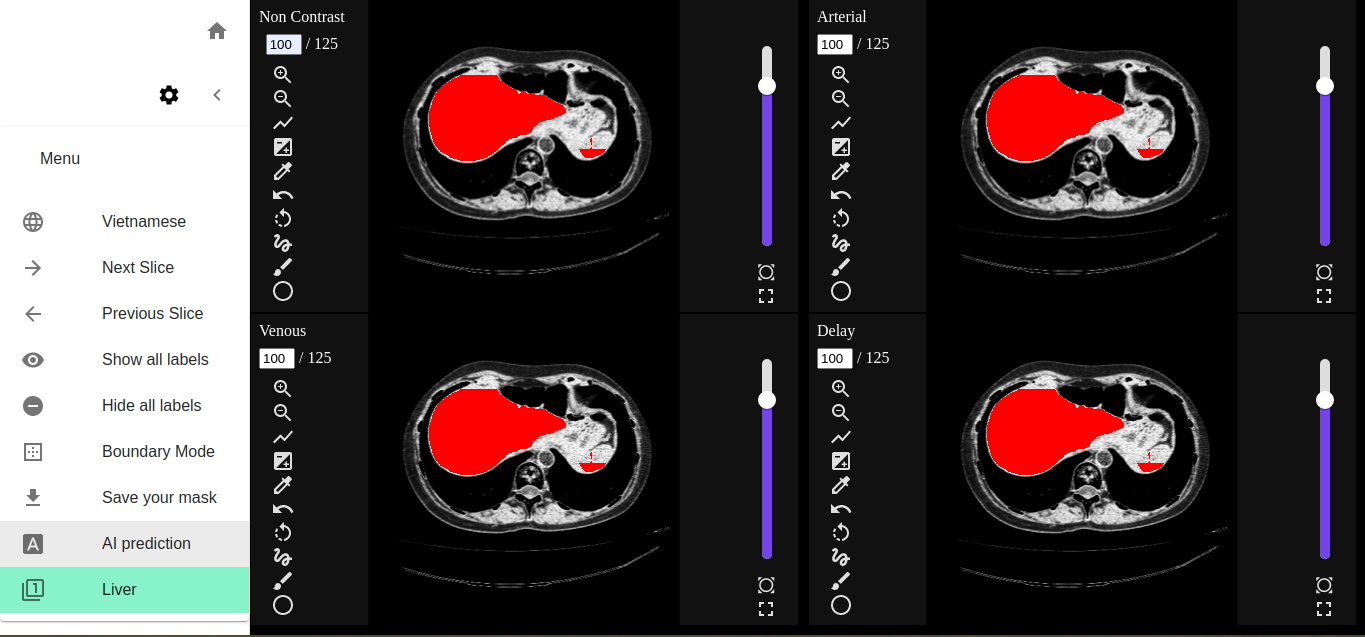
\includegraphics[width=\textwidth]{Medical_CT_poster/images/DAT/user-ui-medical-labeling.png}
        \vspace{-7mm}
        \caption*{Giao diện làm nhãn ảnh y khoa}
        \end{figure}
	\end{minipage}
}

\headerbox{\bf\color{blue} Tài liệu tham khảo}{name=ref, column=0, row=4, below=gui,  span=1}{
    \scriptsize[\textcolor{blue}{1}] O. Ronneberger, P. Fischer, and T. Brox, “U-net: Convolutional networks for biomedical image segmentation,” MICCAI (2015)\\
    \scriptsize[\textcolor{blue}{2}] L.H.Trong, N.V.Hung. “Phát hiện và xây dựng hệ thống mạch máu của gan từ ảnh chụp CT”, LVTN (2019)\\
    \scriptsize[\textcolor{blue}{3}] Qi Dou, H.Chen. “3D Deeply Supervised Network for Automatic Liver Segmentation from CT Volumes”, CoRR (2016)\\
    \scriptsize[\textcolor{blue}{4}] N.Q.Ha, T.Q.Phap, M.D.Tu. “Xây dựng mô hình gan từ ảnh chụp CT”, LVTN (2019)
}

\headerbox{\bf\color{blue} Tổng kết}{name=summary,column=1,row=2,below=experiment_result,span=1,bottomaligned=ref}{
    \textbf{\color{blue} Kết quả đạt được:}
    \begin{itemize}
    \compresslist
    \setlength{\itemindent}{.2in}
	    \item Kết quả phân đoạn hệ số Dice \textbf{60.75\%} trên mạch máu và \textbf{95.83\%} trên gan.
        \item Hoàn thiện hệ thống làm nhãn ảnh y khoa.
	\end{itemize}
	\textbf{\color{blue} Hướng phát triển:}
	\begin{itemize}
	\compresslist
	\setlength{\itemsep}{0pt}%
    \setlength{\parskip}{0pt}
    \setlength{\itemindent}{.2in}
		\item Phân đoạn nhiều cơ quan nội tạng khác nhau.
		\item Trực quan hóa dữ liệu dưới dạng mô hình 3D.
		\item Cải thiện phần tải và hiển thị ảnh DICOM, phần phóng to, thu nhỏ, kéo thả hình ảnh được nhanh hơn. 
	\end{itemize}
}
\end{poster}
\end{document}
